% #############################################################################
% This is Chapter 3
% !TEX root = ../main.tex
% #############################################################################
% Change the Name of the Chapter i the following line
\fancychapter{Autonomous Vehicle Models}
\cleardoublepage
% The following line allows to ref this chapter
\label{chap:autonomousvehiclemodels}

\par In this chapter equations that rule the motion of an autonomous marine vehicle are derived. To this end, the coordinate frames will be defined initially(\ref{sec:refframes}). What follows will be the general vehicle motion equations for the dubin's car (sec:dubincarequations). Finally, the motion equations for the MEDUSA model are presented (the characterization of the vehicle MEDUSA (\ref{sec:medusamodelequations}). The models presented here rely on parameters specific for each vehicle, which will not be discuessed in this chapter.

\par In this chapter we address the mathmatical models that describe the motion of vehicles in 2 dimensional space.


\section{Reference Frames and Notaion}
\label{sec:refframes}


\par To derive the equations of motion for a marine vehicle it is standard practice to define two coordinate frames; Earth-fixed inertial frame $\{U\}$ composed by the orthonormal axes $\{x_U,y_U,z_U\}$ and the body-fixed frame $\{B\}$ composed by the axes $\{x_B,y_B,z_B\}$, as indicated in Figure \ref{fig:coordinate}.

\begin{itemize}
    \item $x_B$ is the longitudinal axis (directed from the stern to fore)
    \item $y_B$ is the transversal axis (directed from to starboard)
    \item $z_B$ is the normal axix (directed from top to bottom)
\end{itemize}

\par To simplify the model equations, the origin of the body-fixed frame is normally chosen to coincide with the centre of mass of the vehicle. The motion control of $\{B\}$ (that corresponds to the motion of the vehicle) is described relative to the intertial frame $\{U\}$.

\par In general, six independent coordinate are necessary to determine the evolution of the position and orientation (six \ac{DOF}), three position coordinates $(x,y,z)$ and using the Euler orientation angles $(\phi, \theta, \psi)$. The six motion components are difined as \textit{surge}, \textit{sway}, \textit{heave}, \textit{roll}, \textit{pitch}, and \textit{yaw}, and adopting the SNAME \footnote{The Society of Naval Architects \& Marine Engineers - http://www.sname.org/} notation it can be written as in the Table \ref{tab:coordinate_notation} or in a vectorial form: 
\begin{itemize}
    \item $\eta_1 = [x,y,z]^T$ - position of the origin of $\{B\}$ with respect to $\{U\}$
    \item $\eta_2 = [\phi, \theta, \psi]^T$ - orientation of $\{B\}$ with respect to $\{U\}$.
    \item $\nu_1 = [u,v,w]^T$ - linear velocity of the origin of $\{B\}$ relative to $\{U\}$, expressed in $\{B\}$.
    \item $\nu_2 = [p,q,r]^T$ - angular velocity of $\{B\}$ relative to $\{U\}$, expressed in $\{B\}$.
    \item $\tau_1 = [X,Y,Z]^T$ - actuating forces expressed in $\{B\}$.
    \item $\tau_2 = [K,M,N]^T$ - actuating moments expressed in $\{B\}$
\end{itemize}
In compact form yields
\begin{equation}
    \begin{cases}
        \eta = [\eta_1^T, \eta_2^T]^T \\
        \nu = [\nu_1^T, \nu_2^T]^T \\
        \tau_{RB} = [\tau_1^T, \tau_2^T]^T
    \end{cases}
\end{equation}

\begin{table}[h!]
\begin{tabular}{|l|l|l|l|}
\hline
\multicolumn{1}{|c|}{Degree of Freedom} &
  \multicolumn{1}{c|}{\begin{tabular}[c]{@{}c@{}}Forces and\\ moments\end{tabular}} &
  \multicolumn{1}{c|}{\begin{tabular}[c]{@{}c@{}}Linear and\\ angular velocities\end{tabular}} &
  \multicolumn{1}{c|}{\begin{tabular}[c]{@{}c@{}}Position and\\ Euler angles\end{tabular}} \\
\hline
1. Motion in the $x$-direction (surge) & $X$ & $u$ & $x$      \\
2. Motion in the $y$-direction (sway)  & $Y$ & $v$ & $y$      \\
3. Motion in the $z$-direction (heave) & $Z$ & $w$ & $z$      \\
4. Rotation about the $x$-axis (roll)  & $K$ & $p$ & $\phi$   \\
5. rotation about the $y$-axis (pitch) & $M$ & $q$ & $\theta$ \\
6. Rotation about the $z$-axis (yaw)   & $N$ & $r$ & $\psi$   \\
\hline
\end{tabular}
\caption{Notation used for marine vehicles}
\label{tab:coordinate_notation}
\end{table}

\par The first step towards describing the motion of an \ac{AUV}

\begin{figure}[h!]
\centering
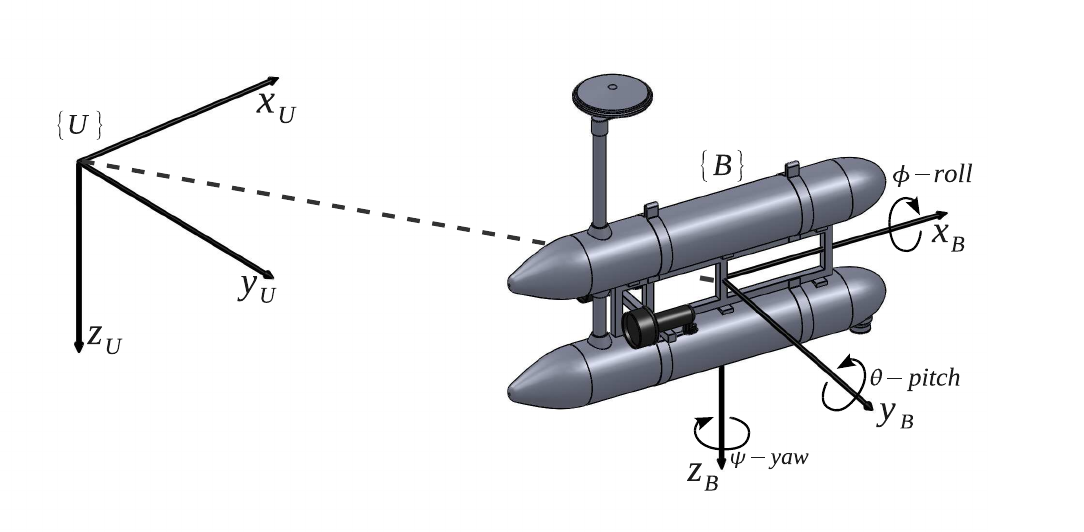
\includegraphics[width=0.8\textwidth]{Images/coordinate_frames.png}
\caption{Coordinate frames}
\label{fig:coordinate}
\end{figure}



\section{Dubin Car}
\label{sec:dubincarequations}

\par In geometry, the term Dubins path typically refers to the shortest curve that connects two points in the two-dimensional Euclidean plane (i.e. x-y plane) with a constraint on the curvature of the path and with prescribed initial and terminal tangents to the path, and an assumption that the vehicle traveling the path can only travel forward \cite{wiki:dubincar}. 
\par A dubin's car is a simple model for a vehicle that transveses a dubin's path.

\par A simple kinematic car model for the systems is: 
\begin{equation}
    \begin{gathered}
        \dot{x} = v \cos \psi \\
        \dot{y} = v \sin \psi \\
        \dot{\psi} = w
    \end{gathered}
\end{equation}
where $(x,y)$ is the car's position, $\psi$ is the car's heading, $v$ is the car's speed, and $w$ is the car's turn rate.

\par The dynamics will be the simplest possible: basic accelerations.
\begin{equation}
    \begin{gathered}
        \dot{w} = r \\
        \dot{v} = a
    \end{gathered}
\end{equation}

\par Is differentially flat \cite{fliess1995flatness}.



\section{Medusa}
\label{sec:medusamodelequations}
\par Is not differentially flat 

\par The kinematics trats only the gemotrical aspects of motion, and relates the velocities with poisiton. Using the coordinate frames notation in Section \ref{sec:refframes}, the kinematic equation can be expressed as
\begin{equation}
    \dot{\eta} = J(\eta)\nu
\end{equation}
with 
\begin{equation}
    J(\eta) = \begin{bmatrix}
        \prescript{U}{B}{R}
    \end{bmatrix}
\end{equation}
where
\begin{equation}
    \prescript{U}{B}{R(\Theta)} = \begin{bmatrix}
        c\psi c\theta & c\psi s\theta s\phi-s \psi c\phi & c\psi s\theta c\phi+s\psi s\phi \\
        s\psi c\theta & s\psi s\theta s\phi+c\psi c\phi & s\psi s\theta c\phi-c\psi s\phi \\
        -s\theta & c\theta s\phi & c\theta c\phi
    \end{bmatrix}, s\cdot = \sin(\cdot), c\cdot=\cos(\cdot)
\end{equation}
is the rotation matrix from $\{B\}$ to $\{U\}$, \cite{fossen2006nonlinear}, defined my means of three successive rotations ($zyx$-convention):

\begin{equation}
    \prescript{U}{B}{R(\Theta)} = R_{z,\psi}R_{y,\theta}R_{x,\phi}
\end{equation}
and
\begin{equation}
    T_{\Theta}(\Theta) = \begin{bmatrix}
        1 & s\phi\ t\theta & c\phi t\theta \\
        0 & c\phi & -s\phi \\
        0 & c\phi / c\theta & c\phi / c\theta 
    \end{bmatrix}, \theta \neq \pm 90º
\end{equation}

is the Euler attitude transformation matrix that relates the body-fixed angular velocities $(p, q, r)$ with the roll($\dot{\phi}$), pitch($\dot{\theta}$) and yaw($\dot{\psi}$) rates. Notice that $T_\Theta(\Theta)$ is not defined for the pitch angle $\theta = \pm90º$, resulting from using Euler angles to describe the vehicle’s motion. To avoid this singularity, one possibility is to use a quaternion representation \cite{fossen2006nonlinear}. However, due to physical restrictions, the vehicle will operate far from this singularity ($\theta\approx 0$ and $\psi \approx 0$) which implies that we can use the Euler representation.


\subsection{Dynamic equations}

Since the hydrodynamic forces and moments have simpler expressions if written in the body frame because they are generated by the relative motion between the body and the fluid, it is convenient to formulate Newton’s law in $\{B\}$ frame. In that case, the rigid-body equation can be expressed as

\begin{equation}
    M_{RB}\dot{\nu} + C_{RB}(\nu)\nu = \tau_{RB}
    \label{eq:rigid_body}
\end{equation}

where $M_{RB}$s the rigid body inertia matrix, $C_{RB}$ represents the Coriolis and centrifugal terms and $\tau_{RB}$ is a generalized vector of external forces and moments and can be decomposed as
 
\begin{equation}
    \tau_{RB} = \tau + \tau_A + \tau_D + \tau_R + \tau_{dist}
    \label{eq:tau_rb}
\end{equation}

where
\begin{enumerate}
    \item $\tau$ - Vector of forces and torques due to thrusters/surfaces which usually can be viewed as the control input
    \item $\tau_A$ + The force and moment vector due to the hydrodynamic added mass,
    \begin{equation}
        \tau_A = - M_A \dot{\nu} - C_A(\nu)\nu
        \label{eq:tau_a}
    \end{equation}
    \item $\tau_D$ - Hydrodynamics terms due to lift, drag, skin friction, etc.
    \begin{equation}
        \tau_D = - D(\nu)\nu
        \label{eq:tau_d}
    \end{equation}
    where $D(\nu)$ denotes the hydrodynamic damping matrix (positive definite).
    \item $\tau_R$ - Restoring forces and torques due to gravity and fluid density,
    \begin{equation}
        \tau_R = -g(\eta)
        \label{eq:tau_r}
    \end{equation}
    \item $\tau_{dist}$ - External disturbances: waves, wind, etc.
\end{enumerate}

\par Replacing \eqref{eq:tau_rb} on \eqref{eq:rigid_body}, taking into account \eqref{eq:tau_a}, \eqref{eq:tau_d}, the dynamic equations can
be written as

\begin{equation}
    \underbrace{M_{RB}\dot{\nu} + C_{RB}(\nu)\nu}_{\text{rigid-body terms}} + \underbrace{M_A(\dot{\nu}) + C_A(\nu)\nu + D(\nu)\nu}_{\text{hydrodynamic terms}} + \underbrace{g(\nu)}_{\text{restoring terms}} = \tau + \tau_{dist}
\end{equation}
which can be simplified to
\begin{equation}
    M\dot{\nu} + C(\nu)\nu + D(\nu)\nu + g(\nu) = \tau + \tau_{dist}
\end{equation}
where $M = M_{RB} + M_a$, $C(\nu) = C_{RB}(\nu) + C_A(\nu)$.

\subsection{Simplified Equations of Motion}

\par This thesis will focus on movement along a 2-D plane, therefor, the dynamics and kinematics can be simplified such that there are only three degrees of freedom $[x,y,\psi]$.
\par The kinematics with take the simpler form 

\begin{equation}
    \begin{gathered}
        \dot{x} = u \cos \psi - v \sin \psi, \\
        \dot{y} = u \sin \psi + v \cos \psi, \\
        \dot{\psi} = r.
    \end{gathered}
\end{equation}

\par $\tau_u$ and $\tau_r$ are the external force in $surge$ (common mode) and the external torque about the $z$-axis (differential mode between thrusters), respectively, which can by obtained by 
\begin{equation}
    \begin{gathered}
        \tau_u = F_{sb} + F_{ps}, \\
        \tau_r = l(F_{ps} - F_{sb})
    \end{gathered}
\end{equation}
where $F_{sb}$ and $F_{ps}$ are the starboard and port-side thruster forces, respectively, and $l$ is the length of the arm with respect to the centre of mass.
\par By neglecting roll, pitch and heave motion, the equations for $(u,v,r)$ without disturbances are
\begin{equation} 
    \begin{gathered}
        m_u\dot{u} - m_v v r + d_u u = \tau_u, \\
        m_v \dot{v} + m_u u r + d_v v = 0, \\
        m_r \dot{r} - m_{ub} u v + d_r r = \tau_r,
    \end{gathered}
    \label{eq:simple_medusa_dyamics}
\end{equation}
where
\begin{equation}
    \begin{gathered}
        m_u = m - X_{\dot{u}} \quad d_u = - X_u - X_{|u|u} |u| \\
        m_v = m - Y_{\dot{v}} \quad d_v = - Y_v - Y_{|v|v}|v| \\
        m_r = I_z - N_{\dot{r}} \quad d_r = - N_r - N_{|r|r}|r| \\
        m_{uv} = m_u - m_v
    \end{gathered}
    \label{eq:medusa_masses_and_drags}
\end{equation}


\par All the previous equations were expressed without considering the influence of external factors like ocean currents. If a constrant irrotational ocean current, $v_c$, is introduces, forming an angle $v = v_r+v_c$, where $u_r$ and $v_r$ are the components of the \acs{AUV} velocity with respect to the current and $u_c$ and $v_c$ are the components of the ocean current velocity in the body frame.
The previous dynamic equations \eqref{eq:simple_medusa_dyamics} become
\begin{equation}
    \begin{gathered}
        m_u\dot{u}-m_v(v_r+v_c)r+d_u u=\tau_u, \\
        m_v\dot{v}+m_u(u_r+u_c) r + d_v v=0, \\
        m_r\dot{r}-m_{ub}(u_r+u_c)(v_r+v_c)+d_r r=\tau_r,
    \end{gathered}
\end{equation}
where the expressions for masses and drags remain the same as in \eqref{eq:medusa_masses_and_drags}.


\subsection{\textit{Differentially flatify}}

\par Actually, the medusa model is differentially flat if $x$, $y$ and $\psi$ are to be considered the flat outputs.

The Remaining variables can be obtained by rearanging the kinematics:
\begin{equation}
\begin{split}
    & \begin{bmatrix}
        \dot{x} \\ \dot{y}
    \end{bmatrix} = 
    \begin{bmatrix}
        \cos(\psi) & - \sin(\psi) \\
        \sin(\psi) & \cos(\psi)
    \end{bmatrix} \cdot
    \begin{bmatrix}
        u \\ v
    \end{bmatrix} \Leftrightarrow  \\
    & \begin{bmatrix}
        u \\ v
    \end{bmatrix} = 
    \begin{bmatrix}
        \cos(\psi) & - \sin(\psi) \\
        \sin(\psi) & \cos(\psi)
    \end{bmatrix}^{-1} \cdot
    \begin{bmatrix}
        \dot{x} \\ \dot{y}
    \end{bmatrix} \Leftrightarrow \\
    & \begin{bmatrix}
        u \\ v
    \end{bmatrix} = 
    \begin{bmatrix}
        \cos(\psi) & \sin(\psi) \\
        - \sin(\psi) & \cos(\psi)
    \end{bmatrix} \cdot
    \begin{bmatrix}
        \dot{x} \\ \dot{y}
    \end{bmatrix}
\end{split}
\end{equation}
and the  inputs from the dynamics:
\begin{equation} 
    \begin{gathered}
        \tau_u = m_u\dot{u} - m_v v r + d_u u , \\
        \tau_r = m_r \dot{r} - m_{ub} u v + d_r r ,
    \end{gathered}
    \label{eq:rearaged_dynamics}
\end{equation}
 
\par These equations will always be valid, however, only for $x$, $y$ and $\psi$ that respect
\begin{equation}
    m_v \dot{v} + m_u u r + d_v v = 0
    \label{eq:onlymandatoryconstraint}
\end{equation}
because this equation is what guarantees $\tau_v = 0$. If $\tau_v \neq 0$, the vehicle will have to be fully actuated for the vehicle to follow it.


\todo{calculation of the limits of acceleration of the medusa model}